\documentclass[letterpaper,12pt]{article}

\usepackage{threeparttable}
\usepackage{geometry}
\geometry{letterpaper,tmargin=1in,bmargin=1in,lmargin=1.25in,rmargin=1.25in}
\usepackage[format=hang,font=normalsize,labelfont=bf]{caption}
\usepackage{amsmath}
\usepackage{multirow}
\usepackage{array}
\usepackage{delarray}
\usepackage{listings}
\usepackage{amssymb}
\usepackage{amsthm}
\usepackage{lscape}
\usepackage{natbib}
\usepackage{setspace}
\usepackage{float,color}
\usepackage[pdftex]{graphicx}
\usepackage{pdfsync}
\usepackage{verbatim}
\usepackage{placeins}
\usepackage{geometry}
\usepackage{pdflscape}
\synctex=1
\usepackage{hyperref}
\hypersetup{colorlinks,linkcolor=red,urlcolor=blue,citecolor=red}
\usepackage{bm}


\theoremstyle{definition}
\newtheorem{theorem}{Theorem}
\newtheorem{acknowledgement}[theorem]{Acknowledgement}
\newtheorem{algorithm}[theorem]{Algorithm}
\newtheorem{axiom}[theorem]{Axiom}
\newtheorem{case}[theorem]{Case}
\newtheorem{claim}[theorem]{Claim}
\newtheorem{conclusion}[theorem]{Conclusion}
\newtheorem{condition}[theorem]{Condition}
\newtheorem{conjecture}[theorem]{Conjecture}
\newtheorem{corollary}[theorem]{Corollary}
\newtheorem{criterion}[theorem]{Criterion}
\newtheorem{definition}{Definition} % Number definitions on their own
\newtheorem{derivation}{Derivation} % Number derivations on their own
\newtheorem{example}[theorem]{Example}
\newtheorem{exercise}[theorem]{Exercise}
\newtheorem{lemma}[theorem]{Lemma}
\newtheorem{notation}[theorem]{Notation}
\newtheorem{problem}[theorem]{Problem}
\newtheorem{proposition}{Proposition} % Number propositions on their own
\newtheorem{remark}[theorem]{Remark}
\newtheorem{solution}[theorem]{Solution}
\newtheorem{summary}[theorem]{Summary}
\bibliographystyle{aer}
\newcommand\ve{\varepsilon}
\renewcommand\theenumi{\roman{enumi}}
\newcommand\norm[1]{\left\lVert#1\right\rVert}

\begin{document}
\subsection*{9.1}




$\mathbf{p}$ being non-zero implies that there exists some non-zero $p_i$. So let $p_n \neq 0$. Remember that \[d = p_1x_1 + ...+ p_{n-1}x_{n-1} + p_nx_n\]

Solving for $x_n$, we get that\[x_n = \frac{d - ( p_1x_1 + ...+ p_{n-1}x_{n-1} )}{p_n}\]


\noindent We can also rewrite $A_1 \mathbf{x} \preceq \mathbf{b_1}$ in the following matrix form \\

$\begin{matrix}
a_{1,1}x_1 +& ...&+a_{1,(n-1)}x_{n-1} &+ a_{1,n}x_{n} \\
a_{2,1}x_1 +& ...&+a_{2,(n-1)}x_{n-1} &+ a_{2,n}x_{n} \\
\vdots & &\vdots &\vdots    \\
a_{n,1}x_1 +& ...&+ a_{n,(n-1)}x_{n-1} &+ a_{n,n}x_{n} \\
\end{matrix}$
$\begin{matrix}
\leq b_1\\
\leq b_2\\
\vdots\\
\leq b_{n}\\
\end{matrix}$\\

Plugging in for $x_n$, we know that we will have some coefficient $c_{1,i}$ in front of each $x_i$ along with a constant $\frac{d}{p_n}$ replacing the $n^{\text{th}}$ $x$ term such that

$\begin{matrix}
    c_{1,1} x_1 + &...& + c_{1,n-1} x_{n-1} & + \frac{d}{p_n} \\
    c_{2,1} x_1 + &...& + c_{2,n-1} x_{n-1} & + \frac{d}{p_n} \\
    \vdots &  &\vdots    \\
    c_{n,1} x_1 + &...& + c_{n,n-1} x_{n-1} & + \frac{d}{p_n} \\
\end{matrix}$
$\begin{matrix}
\leq b_1\\
\leq b_2\\
\vdots\\
\leq b_{n}\\
\end{matrix}$\\

which can also be expressed as 

$\begin{matrix}
    c_{1,1} x_1 + &...& + c_{1,n-1} x_{n-1} &  \\
    c_{2,1} x_1 + &...& + c_{2,n-1} x_{n-1} &  \\
    \vdots & &\vdots    \\
    c_{n,1} x_1 + &...& + c_{n,n-1} x_{n-1} &  \\
\end{matrix}$
$\begin{matrix}
\leq b_1 - \frac{d}{p_n}\\
\leq b_2 - \frac{d}{p_n}\\
\vdots\\
\leq b_{n} - \frac{d}{p_n}\\
\end{matrix}$\\


\noindent We can now rewrite the matrix $A_2$ as vector $\mathbf{b}_2$ like\\
$A_2= 
\begin{bmatrix}
    c_{1,1}   &...& c_{1,n-1} &  \\
    c_{2,1}   &...&  c_{2,n-1} &  \\
    \vdots & &\vdots    \\
    c_{n,1}   &...&  c_{n,n-1} &  \\
\end{bmatrix} \mathbf{x}$   and    $\mathbf{b}_2 = 
\begin{bmatrix}
 b_1 - \frac{d}{p_n}\\
 b_2 - \frac{d}{p_n}\\
\vdots\\
 b_{n} - \frac{d}{p_n}\\
\end{bmatrix} = \mathbf{b}_1 -  \mathbf{\frac{d}{p_n}}$\\

Notice that this matrix is $n \times (n-1)$ and the vectors are $n \times 1$.\\

Note that the right term is a constant, which will go to zero upon maximizing. Then $\mathbf{x}$ will optimize both $c_1x_1 +...+ c_{n-1}x_{n-1}$ and $c_1x_1 +...+ c_{n-1}x_{n-1} + c_nx_n$

And we have that that \[\mathbf{y} = \begin{bmatrix}

x_1\\
\vdots\\
x_{n-1}\\
\end{bmatrix}\] and \[\mathbf{c}_2 = \begin{bmatrix}
c_1\\
\vdots\\
c_{n-1}\\
\end{bmatrix}\] \\

The other solution is an $(n-1) \times 1$ vector $\mathbf{y}^*$. Then the optimum can be written as\\
\[c_1y_1^* +...+ c_{n-1}y_{n-1}^*\]\\

And we get that the first maximization problem can be written as\\
\[c_1x_1 +...+ c_{n-1}x_{n-1} + c_n\alpha = c_1y_1^* +...+ c_{n-1}y_{n-1}^* + c_n\alpha\]\\

Thus we have that  $M$ is a diagonal matrix of 1's except for in the bottom-right corner, and $x_0$ is a vector of zeros excepting the last entry.

\subsection*{9.2}


Let $g$ and $k$ be the number of GI Barb and Kennie dolls, respectively. Subtracting the cost function from the revenue function, we have the profit function  \[\pi = 4g + 3k \quad k \geq 0, g \geq 0, 15g + 10k \leq 1800, k + g \leq 150\]
Now if we have that \[
\mathbf{c} = 
\begin{bmatrix}
4 \\ 3 
\end{bmatrix}
\quad \mathbf{d} = 
\begin{bmatrix}
   g \\ k 
\end{bmatrix}
A = 
\begin{bmatrix}
    15 & 10 \\ 1 & 1
\end{bmatrix}
\mathbf{b} = 
\begin{bmatrix}
    1800 \\ 150
\end{bmatrix}
\]
constrained by \[ A \mathbf{d} \leq \mathbf{b}, \mathbf{d} \succeq 0 \]
We have our problem
\begin{align*}
\underset{}{\text{maximize}} \qquad &\mathbf{c}^T \mathbf{d}\\
\text{s.t.} \qquad &A \mathbf{d} \preceq \mathbf{b}
\end{align*}




\subsection*{9.3}

We want to 
\[\underset{}{\text{minimize}} \qquad ||Ax - \mathbf{b}||_1\]
We know that 
\begin{align*}
||Ax - \mathbf{b}||_1 &= 
\left|\left|
\begin{bmatrix}
    a_{11} & a_{21}& \cdots& a_{1m} \\
    a_{21} & a_{22}& \ldots& a_{2m} \\
    \vdots& \vdots& \ddots & \vdots \\
    a{m1}& \cdots& \cdots & a{mn} 
\end{bmatrix}
\begin{bmatrix}
    x_1\\
    x_2\\
    \vdots\\
    x_n
\end{bmatrix}
-
\begin{bmatrix}
    b_1\\
    b_2\\
    \vdots\\
    b_m
\end{bmatrix}
\right|\right|_1
\\
 &= 
\left|\left|
\begin{bmatrix}
    a_{11}x_1 +  \cdots + a_{1n}x_n -b_1\\
    a_{21}x_1 +  \cdots + a_{2n}x_n -b_2\\
    \vdots\\
    a_{m1}x_1 +  \cdots + a_{mn}x_n -b_m\\
\end{bmatrix}
\right|\right|_1\\
 &= |a_{11}x_1 +  \cdots + a_{1n}x_n -b_1| + \cdots + |a_{m1}x_1 +  \cdots + a_{mn}x_n -b_m|
\end{align*}


The linear program that achieves the same aim is as follows:
\\The absolute value is not a linear operator, so we need to find a different objective function than the one given above. To find such an objective function, we know that the difference between $Ax$ and $\mathbf{b}$ is equal to some $\mathbf{s} \in \mathbb{R}^{2m}$, the odd elements of the vector corresponding to the case where this difference is negative, and the even elements corresponding to the case where this difference is positive. For each $i^\text{th}$ element of $Ax-\mathbf{b}$, let the constraints be given as follows:
\begin{align*}
    a_{i1}x_1 +  \cdots + a_{in}x_n - s_{2i-1} \leq b_i\\
    a_{i1}x_1 +  \cdots + a_{in}x_n + s_{2i} \geq b_i\\
    x_1, \cdots, x_n \geq 0\\
    s_1, \cdots, s_{2m} \geq 0
\end{align*}

And we have our final step:
\begin{align*}
\underset{x,s}{\text{minimize}} \qquad &\mathbf{1}^T \mathbf{s} \\ 
\text{s.t.}\qquad & Ax -\mathbf{s}_{\text{odds}}  \preceq b\\
& Ax+\mathbf{s}_{\text{evens}} \succeq b
\end{align*}

Now let 
\[c = 
\begin{bmatrix}
    0 & \cdots & 0 & 1 & \cdots & 1
\end{bmatrix}\\\quad 
y = 
\begin{bmatrix}
x_1 \\ 
\vdots \\ x_n \\ s_1 \\ \vdots \\ s_{2m}
\end{bmatrix}
\\ \quad A = 
\begin{bmatrix}
    A & I \\ -A & I
\end{bmatrix}
\\ \quad b  = 
\begin{bmatrix}
    b\\-b
\end{bmatrix}
\]
Then we have the problem
\begin{align*}
\underset{x,s}{\text{minimize}} \qquad & c^T \mathbf{y}\\
\text{s.t.} \qquad & A \mathbf{y} \succeq \mathbf{b}
\end{align*}
Now the first $n$ entries of $y^*$ will be $x^*$


\subsection*{9.5 (i)}

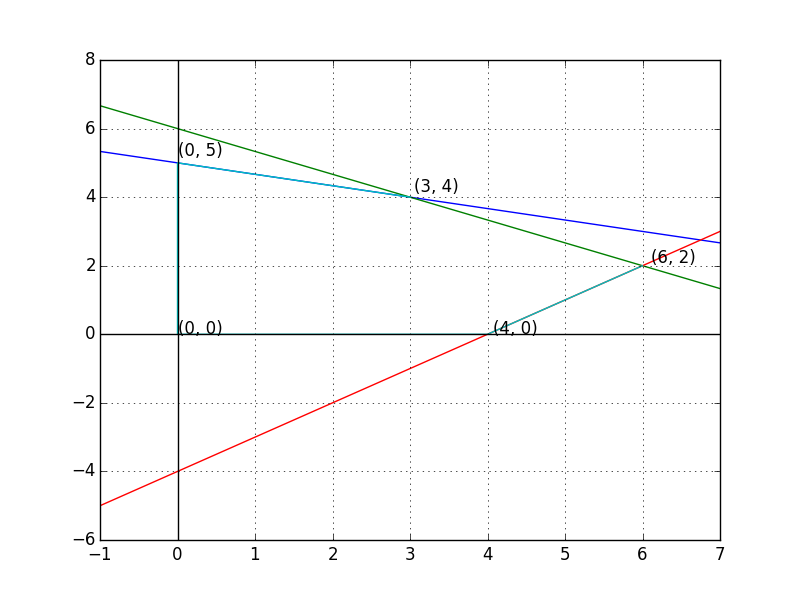
\includegraphics[scale = .75]{first95}
Values are as follows:

0 for (0,0)\\
5 for (0,5)\\
12 for (4,0)\\
13 for (3,4)\\
20 for (6,2)\\

\[ \text{Optimal value} = 20 \qquad x_1 = 6 \qquad x_2 = 2\]

\subsection*{9.5 (ii)}

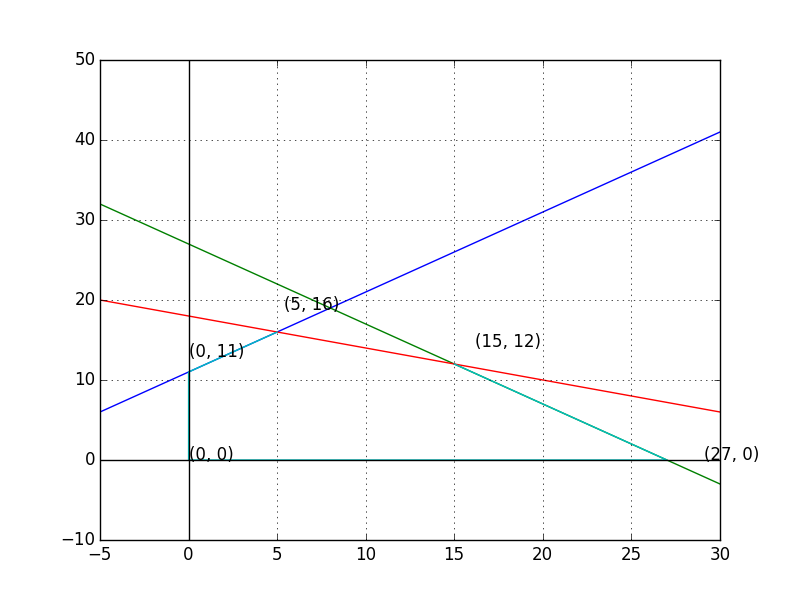
\includegraphics[scale = .75]{second95}

\[ \text{Optimal value} = 132 \qquad x = 15 \qquad y = 12\]

\subsection*{9.6(i)}

\[
\begin{bmatrix}
 -3 & -1 & 0 & 0 & 0 &  0 \\
  1 &  3 & 1 & 0 & 0 & 15 \\
  2 &  3 & 0 & 1 & 0 & 18 \\
  1 & -1 & 0 & 0 & 1 &  4 \\
\end{bmatrix}
\]
\[
\begin{bmatrix}
 0 & -4 & 0 & 0 &  3 & 12 \\
 0 &  4 & 1 & 0 & -1 & 11 \\
 0 &  5 & 0 & 1 & -2 & 10 \\
 1 & -1 & 0 & 0 &  1 &  4 \\
\end{bmatrix}
\]
\[
\begin{bmatrix}
 0 & 0 & 0 &  0.8 &  1.4 & 20 \\
 0 & 0 & 1 & -0.8 &  0.6 &  3 \\
 0 & 5 & 0 &  1   & -2   & 10 \\
 1 & 0 & 0 &  0.2 &  0.6 &  6
\end{bmatrix}
\]

\[ \text{Optimal value} = 20 \qquad x_1 = 6 \qquad x_2 = 2\]

\subsection*{9.6 (ii)}
\[
\begin{bmatrix}
 -4 & -6 & 0 & 0 & 0 &  0 \\
 -1 &  1 & 1 & 0 & 0 & 11 \\
  1 &  1 & 0 & 1 & 0 & 27 \\
  2 &  5 & 0 & 0 & 1 & 90 \\
\end{bmatrix}
\]
\[
\begin{bmatrix}
 0 & -2 & 0 &  4 & 0 & 108 \\
 0 &  2 & 1 &  1 & 0 &  38 \\
 1 &  1 & 0 &  1 & 0 &  27 \\
 0 &  3 & 0 & -2 & 1 &  36 \\
\end{bmatrix}
\]
\[
\begin{bmatrix}
 0 & 0 & 0 &  2.66667 &  0.666667 & 132 \\
 0 & 0 & 1 &  2.33333 & -0.666667 &  14 \\
 1 & 0 & 0 &  1.66667 & -0.333333 &  15 \\
 0 & 3 & 0 & -2       &  1        &  36 \\
\end{bmatrix}
\]

\[ \text{Optimal value} = 132 \qquad x = 15 \qquad y = 12\]

\subsection*{9.7}
\[
\begin{bmatrix}
-4 & -3 & 0 & 0 &    0 \\
 15 & 10 & 1 & 0 & 1800 \\
  1 &  1 & 0 & 1 &  150 \\
\end{bmatrix}
\]
\[
\begin{bmatrix}
  0 & -0.333333 &  0.266667  & 0 &  480 \\
 15 & 10        &  1         & 0 & 1800 \\
  0 &  0.333333 & -0.0666667 & 1 &   30 \\
\end{bmatrix}
\]
\[
\begin{bmatrix}
  0 & 0        &  0.2       &   1 & 510 \\
 15 & 0        &  3         & -30 & 900 \\
  0 & 0.333333 & -0.0666667 &   1 &  30 \\
\end{bmatrix}
\]
\[ \text{Optimal profit} = 510 \qquad g = 60 \qquad k = 90\]
\subsection*{9.8 (i)}
As there is a negative in the $\mathbf{b}$ column, we want to try to solve the auxillary problem. We proceed as follows:
\[
\begin{bmatrix}
0&0&0&0&0&1&0 \\
-1&-2&0&0&0&0&0 \\
-4&-2&1&0&0&-1&-8 \\
-2&3&0&1&0&0&6 \\
1&0&0&0&1&0&3 \\
\end{bmatrix}
\]
\[
\begin{bmatrix}
-4&-2&1&0&0&0&-8 \\
-1&-2&0&0&0&0&0 \\
-4&-2&1&0&0&-1&-8 \\
-2&3&0&1&0&0&6 \\
1&0&0&0&1&0&3 \\
\end{bmatrix}
\]
\[
\begin{bmatrix}
0&-2&1&0&4&0&4 \\
0&-2&0&0&1&0&3 \\
0&-2&1&0&0&-1&4 \\
0&3 &0&1&0&0&12 \\
1&0 &0&0&1&0&3 \\
\end{bmatrix}
\]
\[
\begin{bmatrix}
0&0&1&\frac{2}{3}&4&0&12 \\
0&0&0&\frac{2}{3}&1&0&11\\
0&0&1&\frac{2}{3}&0&-1&12 \\
0&3&0&1          &0&0&12 \\
1&0&0&0          &1&0&3 \\
\end{bmatrix}
\]
\\
As there are no negative values that remain in the top row and there is a non-zero entry in the optimal value slot, we know that the problem is infeasible.

\subsection*{9.8 (ii)}

As there is a negative in the $\mathbf{b}$ column, we want to try to solve the auxillary problem. We proceed as follows:
\[
\begin{bmatrix}
0&0&0&0&0&1&0 \\
5&2&0&0&0&0&0 \\
5&3&1&0&0&0&15 \\
3&5&0&1&0&0&15 \\
4&-3&0&0&1&-1&-12 \\
\end{bmatrix}
\]
\[
\begin{bmatrix}
4&-3&0&0&1&0&-12 \\
5&2&0&0&0&0&0 \\
5&3&1&0&0&0&15 \\
3&5&0&1&0&0&15 \\
4&-3&0&0&1&-1&-12 \\
\end{bmatrix}
\]
\[
\begin{bmatrix}
\frac{12}{5}&0&0&\frac{3}{5}&1&0&-3 \\
\frac{19}{5}&0&0&-\frac{2}{5}&0&0&-6 \\
\frac{16}{5}&0&1&-\frac{3}{5}&0&0&6 \\
3&5&0&1&0&0&15 \\
\frac{29}{5}&0&0&\frac{3}{5}&1&-1&-3 \\
\end{bmatrix}
\]
\\
As there are no negative values that remain in the top row and there is a non-zero entry in the optimal value slot, we know that the problem is infeasible.

\subsection*{9.8 (iii)}
\[
\begin{bmatrix}
 3 & -1 & 0 & 0 & 0 \\
  0 &  1 & 1 & 0 & 4 \\
 -2 &  3 & 0 & 1 & 6 \\
    
\end{bmatrix}
\]
\[
\begin{bmatrix}
  2.33333  & 0 & 0 &  0.333333 & 2 \\
  0.666667 & 0 & 1 & -0.333333 & 2 \\
 -2        & 3 & 0 &  1        & 6 \\
    
\end{bmatrix}
\]
 
\[ \text{Optimal value} = 2 \qquad x_1 = 0 \qquad x_2 = 2\]


\subsection*{9.9}


\begin{align*}
\displaystyle \max_{x, y, z} \qquad &-x +y +z\\ 
 \text{s.t.} \qquad  &x\leq 2\\
&y+z \leq 2\\
\end{align*}
This works because the objective function is maximized by minimizing x, and
x is unbounded in the positive direction.\\

\subsection*{9.10}


\begin{align*}
\displaystyle \max_{x, y, z} \qquad &x +y +z\\ 
\text{s.t.} \qquad &x\leq 2\\
&y+z \leq 2\\
\end{align*}
This works because the objective function is maximized by maximizing x, and
x is unbounded in the positive direction.\\

\subsection*{9.11}


\begin{align*}
\displaystyle \max_{x, y, z} \qquad &x +y +z\\ 
\text{s.t.} \qquad &-x-z \leq -2\\
&-y-z \leq -2\\
\end{align*}
This objective function is all negative, so maximizing will be pushing to
infinity all directions.\\

\subsection*{9.12}


\begin{align*}
\displaystyle \max_{x_1, y_1, z_1} \qquad &x_1  +y_1 +z_1\\ 
\text{s.t.} \qquad &x_1+z_1+1 \leq 2\\
&y_1+z_1 \leq 2\\
&-z_1 \leq -1
\end{align*}

\[x_1 = x_2, y_1 = y_2, z_1 = z_2+1\] Thus we have that \\
\begin{align*}
\displaystyle \max_{x_2, y_2, z_2} \qquad &x_2  +y_2 +z_2\\ 
\text{s.t.} \qquad &-x_2+-z_2-1 \leq -2\\
&-y_1+-z_1 \leq 2\\
&-z_2 \leq -2
\end{align*}

\subsection*{9.13}
\begin{align*}
\begin{bmatrix}
-10&  57&   9&  24&   0&   0&   0&   0&\\
  0.5&  -5.5  &-2.5 &  9&   1&   0&   0&   0&\\
  0.5&  -1.5 & -0.5  & 1&   0&   1&   0&   0&\\
  1&   0&   0&   0&   0&   0&   1&   1&
\end{bmatrix}
\end{align*}

\begin{align*}
\begin{bmatrix}
  0&  57&   9&  24&   0&   0&  10&  10&\\
  0&  -5.5&  -2.5   &9&   1&   0&  -0.5  &-0.5\\
  0&  -1.5 & -0.5 &  1&   0&   1&  -0.5&  -0.5\\
  1&   0&   0&   0&   0&   0&   1&   1&\\
\end{bmatrix}
\end{align*}
 
\[ \implies x_1 = 1 \quad  x_2 = 0 \quad x_3 = 0 \quad x_4 = 0  \quad \text{Optimal value} = 10\]

\subsection*{9.14}

The first entry of the right-most column is the optimal value of a function after having applied the simplex algorithm. In this case, that all the other entries of the last column are zeros, whatever is in the upper right hand corner of the matrix will be the final optimal value as the only way it could change is by adding a non-zero row to it according to the simplex algorithm. It won't change when adding zeros to it, though, so this is the optimal value. The only other case would be if there were no answer, in which case it would be unbounded.

\subsection*{9.15 (i)}
No. Suppose to the contrary that there is such a case in which a zero appears in the last column. For this to be true, there would have to be four entries $a,b,c,d$ in a matrix $A$ such that
\[A = 
\begin{bmatrix}
    & & & \\
    a & & & b\\
    c & & & d\\
\end{bmatrix}
\text{and that}\qquad
b = \frac{a}{c}d
\]
However, this would suggest that \[\frac{b}{a} = \frac{d}{c}\]
Now, we supposed that there was never a tie for the choice of leaving variable, meaning that \[\frac{b}{a} \neq \frac{d}{c} \]
We have, then a contradiction. 

\subsection*{9.15 (ii)}
No it cannot cycle. The only time such a problem can cycle is if the optimal value stays the same. In this problem, though, we know that there are never any zeros in the b column by (i), meaning that the optimal value will change with every iteration and therefore will never cycle.

\subsection*{9.16}

By definition, we have that
\begin{align*}
\\ \textbf{c}^T \textbf{x} &= \textbf{x}^T \textbf{c}
\\ &\preceq \textbf{x}^T(A^T\textbf{y})
\\ &= (A\textbf{x})^T \textbf{y}
\\ &\preceq \textbf{b}^T \textbf{y}
\end{align*}
\\
\\
\subsection*{9.17}


\begin{align*}
\underset{}{\text{maximize}} \qquad &x_1 + 2x_2 + x_3\\
\\ \text{s.t.}  \qquad &x_1 + x_2 + 2x_3 \leq 4
\\  \qquad	&x_1,x_2,x_3 \geq 0
\end{align*}
\\ Then we can express the dual as follows:
\begin{align*}
\underset{}{\text{minimize}} \qquad &4y_1
\\ \text{s.t.} \qquad &y_1 \geq 1\\ &y_1 \geq 2 \\&2y_1 \geq 1\\&y_1 \geq 0
\end{align*}
We have a lower bound of zero for $x_1 = x_2 = x_3 = 0$. As for an upper bound, we have an infinite set of upper bounds, namely, all $y_1 \geq 2, ~ y_1 \in \mathbb{N}$. Let an/the upper bound, then, be $12$ where $y_1 = 3$.
\\
\\

\subsection*{9.18}


We know that the primal form of the linear program can be expressed as follows:
\begin{align*}
\underset{}{\text{maximize}} \qquad &\mathbf{c}^T \mathbf{x}\\
\text{s.t.} \qquad & A\textbf{x} \preceq \textbf{b}
\\& \mathbf{x} \succeq \mathbf{0}
\end{align*}
The dual of this is as follows:
\begin{align*}
\underset{}{\text{maximize}} \qquad &\textbf{b}^T \textbf{y}\\
\text{s.t.} \qquad & A^T\textbf{y} \succeq \mathbf{c}\\ &\textbf{y} \succeq \mathbf{0}
\end{align*}
Standardizing this yields
\begin{align*}
\underset{}{\text{maximize}} \qquad &-\textbf{b}^T \mathbf{y}\\
\text{s.t.} \qquad &-A^T \textbf{y} \preceq -\mathbf{c} \\ &\mathbf{y} \succeq \mathbf{0}
\end{align*}
The dual of this is as follows:
\begin{align*}
\underset{}{\text{minimize}} \qquad &-\mathbf{c}^T\textbf{z}\\
\text{s.t.} \qquad &-A\textbf{z} \succeq -\textbf{b}\\&\textbf{z} \succeq \mathbf{0}
\end{align*}
\\ where $\mathbf{x} = \mathbf{z}$
Standardizing this yields
\begin{align*}
\underset{}{\text{maximize}} \qquad &\mathbf{c}^T \textbf{z}\\
\text{s.t.}\qquad &A\textbf{z} \preceq \textbf{b}
\\\qquad &\mathbf{z} \succeq \mathbf{0}
\end{align*}


\subsection*{Exercise 19}
\[
\begin{bmatrix}
 -1 & -1 & 0 & 0 & 0 & 0 \\
  2 &  1 & 1 & 0 & 0 & 3 \\
  1 &  3 & 0 & 1 & 0 & 5 \\
  2 &  3 & 0 & 0 & 1 & 4 \\
\end{bmatrix}
\]
\[
\begin{bmatrix}
 0 & -0.5 &  0.5 & 0 & 0 & 1.5 \\
 2 &  1   &  1   & 0 & 0 & 3   \\
 0 &  2.5 & -0.5 & 1 & 0 & 3.5 \\
 0 &  2   & -1   & 0 & 1 & 1   \\
\end{bmatrix}
\]
\[
\begin{bmatrix}
 0 & 0 &  0.25 & 0 &  0.25 & 1.75 \\
 2 & 0 &  1.5  & 0 & -0.5  & 2.5  \\
 0 & 0 &  0.75 & 1 & -1.25 & 2.25 \\
 0 & 2 & -1    & 0 &  1    & 1    \\
\end{bmatrix}
\]





Next we want to solve the dual problem, which is as follows:\\
\[
\begin{bmatrix}
3 & 5& 4& 0& 0& 0 \\
-2&-1&-2& 1& 0& -1 \\
-1&-3&-3& 0& 1& -1 \\
\end{bmatrix}
\]
\[
\begin{bmatrix}
0&0&0&0&0&1&1&0 \\
3&5&4&0&0&0&0&0 \\
-2&-1&-2& 1& 0& -1&0&-1 \\
-1&-3&-3& 0& 1& 0 &-1&-1 \\
\end{bmatrix}
\]\[
\\
\begin{bmatrix}
-3&-4&-2&1&1&0&0&-2\\
3&5&4&0&0&0&0&0 \\
-2&-1&-2& 1& 0& -1&0&-1 \\
-1&-3&-3& 0& 1& 0 &-1&-1 \\
\end{bmatrix}
\]
\[
\begin{bmatrix}
0&\frac{5}{2}&1&- \frac{1}{2}&1& \frac{3}{2} &0& - \frac{1}{2} \\
0&\frac{7}{2}&1&\frac{3}{2}&0&-\frac{3}{2}&0&-\frac{3}{2} \\
-2&-1&-2& 1& 0& -1&0&-1 \\
0&-\frac{5}{2}&-2&-\frac{1}{2}&1&\frac{1}{2}&-1&-\frac{1}{2} \\
\end{bmatrix}
\]
\[
\\
\begin{bmatrix}
0&5&3&0&0&1&1&0\\
0&4&-5&0&3&0&-3&-3 \\
-2&-6&-6&0&2&0&-2&-2 \\
0&-\frac{5}{2}&-2&-\frac{1}{2}&1&\frac{1}{2}&-1&-\frac{1}{2} \\
\end{bmatrix}
\]
\[
\begin{bmatrix}
0&4&-5&0&3&-3 \\
-2&-6&-6&0&2&-2 \\
0&-\frac{5}{2}&-2&-\frac{1}{2}&1&-\frac{1}{2} \\
\end{bmatrix}
\]
\\
\[
\begin{bmatrix}
0&\frac{41}{4}&0&\frac{5}{4}&\frac{1}{2}&-\frac{7}{4} \\
-2&\frac{3}{2}&0&\frac{3}{2}&-1&-\frac{1}{2} \\
0&-\frac{5}{2}&-2&-\frac{1}{2}&1&-\frac{1}{2} \\
\end{bmatrix}
\]
\\
The optimal value, as is apparent, is the same in both the primal and the dual problems, namely $1.75$.

\subsection*{Exercise 20}
(i) \\
By 9.5 (i) we have that 
\[x_1 = 6, x_2 = 2, s_1 = 3, s_2 = 0, s_3 = 0\]
From complementary slackness, we have that for the dual problem 
\[y_1 = 0, w_1 = 0, w_2 = 0\] 
As the slack variables are zero, we know that the constraints' inequalities become equalities and we have that:
\[2y_2 + y_3 = 3 \]
\[3y_2 - y_3 = 1\]
\[\implies y_2 = \frac{4}{5}, y_3 = \frac{7}{5}\]
\\

By 9.5 (ii) we have that \[x_1 = 15, x_2 = 12, s_1 = 14, s_2 = 0, s_3 = 0\]
By complementary slackness we know that for the dual problem \[y_1 = 0, w_1 = 0, w_2 = 0\]
$w_1 \text{and} w_2$ being slack variables for the dual problem. As the slack variables are zero, we know that the constraints' inequalities become equalities and we have that:
\[y_2 + 2y_3 = 4 \]
\[y_2 + 5y_3 = 6\]
\[ \implies y_2 = \frac{8}{3}, y_3 = \frac{2}{3}\]

\subsection*{9.21}

Considering the arc length formula we have
\[\int_a^b \sqrt{1+(y')^2}dx\]
Now let
\[f=\int_a^b \sqrt{1+(y')^2}dx\]
Note that
\[\frac{df}{dx}=0, \frac{df}{dy}=0, \frac{df}{dy'}=\frac{y'}{\sqrt{1+y'^2}}\]
So by the Euler-Langrange equation, we have that
\[\frac{dF}{dy}-\frac{d}{dx}\left(\frac{df}{dy}\right)=0\]
Plugging in, we get
\[0-\frac{d}{dx}\left(\frac{y'}{\sqrt{1+y'^2}}\right)=0\]
Upon integrating both sides we have that
\[c = \frac{y'}{\sqrt{1+y'^2}}\]
Solving for $y'$, we get
\[y'=c\sqrt{1+y'^2}\]\[ \implies y'^2=c^2\left(1+y'^2\right)\]\[ \implies y'^2=c^2+(cy')^2\]
\[\implies y'^2(1-c^2)=c^2 \]\[\implies y'^2=\frac{c^2}{1-c^2} \]\[\implies y'=\sqrt{\frac{c^2}{1-c^2}}\]
now taking the integral with respect to $x$ yields
\[y=\sqrt{\frac{c^2}{1-c^2}}x+b\]
yielding a straight line.\\

\subsection*{9.22}

We are given the equation
\[u(c)=\int_0^T e^{-\beta t}u(c(t))dt\]
we know that $u(c(t))=2\sqrt{c(t)}$ and $c(t)=rk(t)-k'(t)$ so plugging it in we get
\[u(c)=\int_0^T e^{-\beta t}2\sqrt{rk(t)-k'(t)}dt\]
We use the Euler-Lagrange equation
\[L_k(t,k,k')-\frac{d}{dt}L_{k'}(t,k,k')\]
and take $L_k(t,k,k')$ and $L_{k'}(t,k,k')$ of $u(c)$ and plug it into the Euler-Lagrange equation:
\[re^{-\beta T}\left(rk(t)-k'(t)\right)^{\frac{-1}{2}}-\frac{d}{dt}\left[-e^{-\beta t}\left(rk(t)-k'(t)\right)^{-1/2}\right]=0\]
we now differentiate the second part with respect to $t$ and get
\[r-\beta - \frac{1}{2}\left(rk(t)-k'(t)\right)^{-1}\left(rk'(t)-k''(t)\right)=0\]
\[\implies r-\beta=\frac{rk'(t)-k''(t)}{2rk(t)-k'(t)}\]
\[\implies (r-\beta)(rk(t)-k'(t))=\frac{1}{2}(rk'(t)-k''(t))\]
\[\implies (r- \beta)rk(t)-(r-\beta)k'(t)=\frac{1}{2}rk'(t)-\frac{1}{2}k''(t)\]
\[\implies \frac{1}{2}k''(t)-(\frac{3}{2}r-\beta))k'(t)+(r-\beta)rk(t)=0\]
We set the different values of $k$ equal to the following values
\[k=e^{\gamma t}\]
\[k'=\gamma e^{\gamma t}\]
\[k''=\gamma^2 e^{\gamma t}\]
we know plug them into our equation getting
\[\implies \frac{1}{2}\gamma^2 e^{\gamma t}-(\frac{3}{2}r-\beta))\gamma e^{\gamma t}+(r-\beta)re^{\gamma t}=0\]
\[\implies \frac{1}{2}\gamma^2 -(\frac{3}{2}r-\beta))\gamma +(r-\beta)r=0\]
We use the quadratic formula to solve for $\gamma$
\[\frac{3}{2}r-\beta \pm \frac{\sqrt{(\frac{-3}{2}+\beta)^2-2(r-\beta)}}{2(\frac{1}{2})}\]
Simplifying we get
\[\frac{3}{2}r-\beta \pm \sqrt{\frac{9}{4}-\beta +\beta^2 - 2r}\]
so 
\[\gamma_1=\frac{3}{2}r-\beta +\sqrt{\frac{9}{4}-\beta +\beta^2 - 2r}\]
\[\gamma_2=\frac{3}{2}r-\beta -\sqrt{\frac{9}{4}-\beta +\beta^2 - 2r}\]
Now if we let \[\beta = .95 \qquad r = .05 \qquad A = 1 \qquad T = 1 \]
then we get that 



From $\gamma_1 ~ \text{and} ~ \gamma_2$, we have that 
\[y \approx c_1e^{0.726756847964 t} + c_2e^{-2.47675684796 t}\] 
and from our initial condition we have that \[k(0) = A \qquad k(T) = 0\]
which yields a system of equations by which we can solve for $c_1, c_2$
\[
A \approx c_1e^{(0.726756847964) 0} + c_2e^{(-2.47675684796) 0}
\]
\[
0 \approx c_1e^{(0.726756847964) T} + c_2e^{(-2.47675684796) T}
\]

Solving this system of equations gives 

\[ 
c_1 \approx -0.0423390071611 \qquad
c_2 \approx 1.04233900716
\]


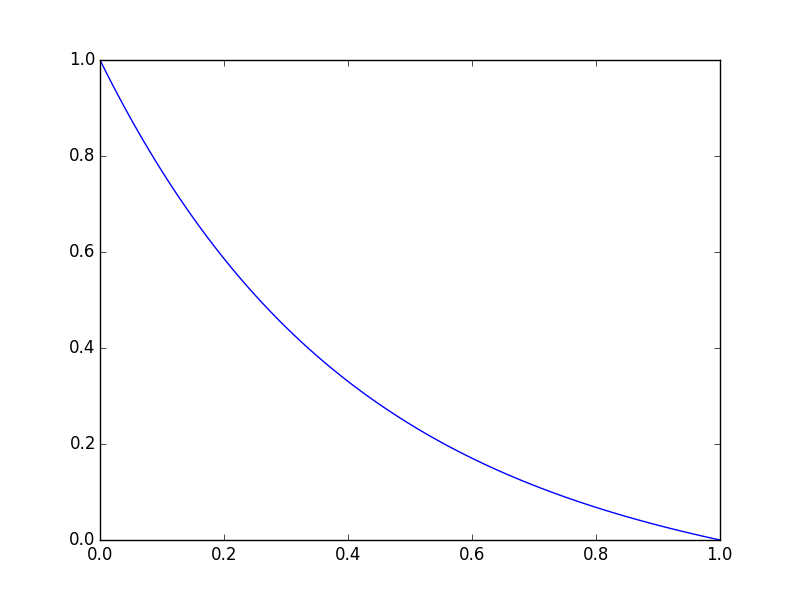
\includegraphics[scale = .75]{problem922}

\end{document}


